\subsection{Oscillatore a ponte di Wien}

\begin{wrapfigure}[6]{r}{0.45\textwidth}
\centering
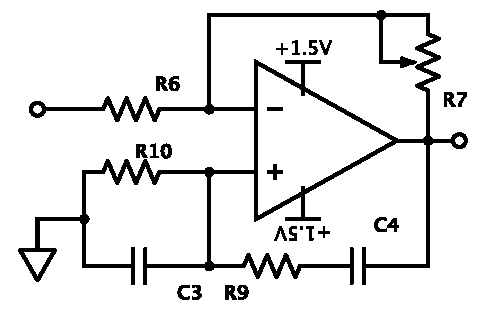
\includegraphics[width=.35\textwidth]{../E08/latex/osc.pdf}
\caption{Schema dell'oscillatore a ponte di Wien senza regolazione del guadagno?}
\label{cir8:without_lamp}
\end{wrapfigure}

\begin{wrapfigure}[6]{r}{0.45\textwidth}
\centering
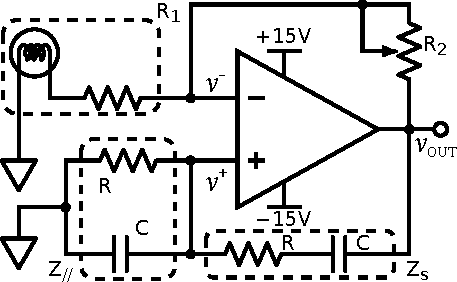
\includegraphics[width=.35\textwidth]{../E08/latex/osc_w_lamp.pdf}
\caption{Schema dell'oscillatore a ponte di Wien con regolazione del guadagno ottenuta mediante una lampadina ad incandescenza}
\label{cir8:with_lamp}
\end{wrapfigure}
